\chapter{Robot Vision II: Camera Calibration}



\section{Important}
Read the entire lab before starting and especially the ``Grading" section so you are aware of all due dates and requirements associated with the lab.  There will be only one online session for this lab, so it is important that you prepare for that one opportunity to work with your TA.

\section{Scope}
\begin{itemize}
    \item Camera Calibration - Obtain the relation between camera and world reference frame
    \item Robot-Camera Calibration - Obtain the mapping between the camera and robot coordinates
    \item Image-Guided Manipulation - Plan and execute path for manipulation task
\end{itemize}    

\section{Objectives}

This is the capstone lab of the semester and will integrate your work done in previous labs with python, ROS, and forward and inverse kinematics.  It will also introduce you to some basic OpenCV techniques.  In this lab you will:
\begin{itemize}
	\item Use OpenCV functions to distinguish the shape of the blocks and find the centroid and angle of them.
	\item Develop transformation equations that relate pixels in the image to coordinates in the world frame
	\item Report the world frame coordinates $(x_w,y_w)$ of the centroid of each block in the camera’s view.
	\item Move the block to a predefined position in the robot's work area.
\end{itemize}


\section{Background}
\subsection{The Camera Model and Calibration Process}
    Robotic systems commonly rely on visual information from the surrounding to perceive
the environment. The source of this information typically comes in the form of images
depicting the scene of the camera views. Therefore, camera can be an extremely useful
sensing device to provide a robotic system with control feedback and perception. Like many
other sensors, there is usually a need to map the acquired signal (imagery) to measurement
(spatial) through a calibration process based on a camera model. The central projection
camera model as shown in \figref{lab6model} is a representation of the image formation process relating
points in world coordinates to their projection on a virtual image plane.
\begin{figure}
	\centering
		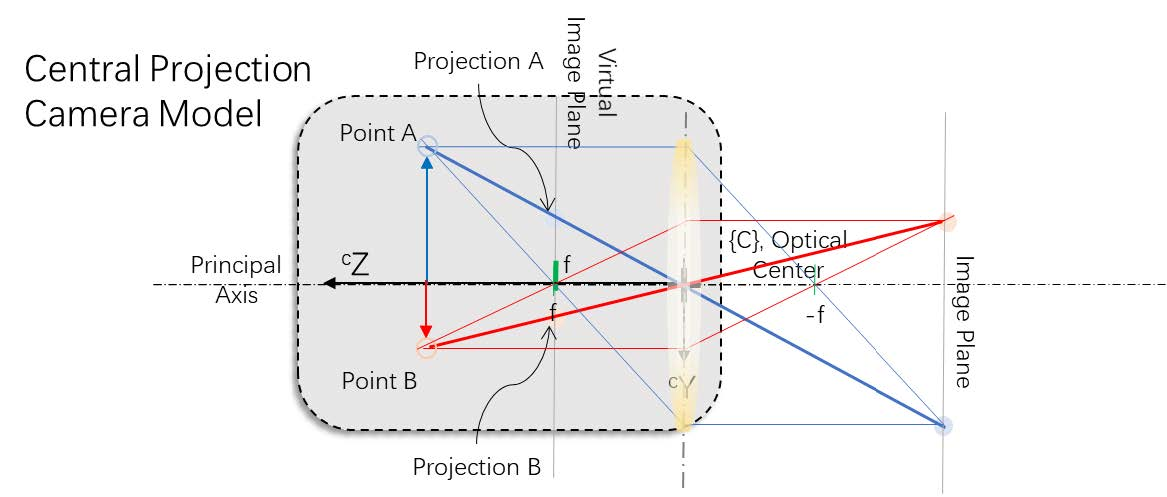
\includegraphics[scale=1]{image/lab7_camera.jpg}
	\caption{\figlbl{lab6model} Central Projection Camera Model}
\end{figure}

Camera calibration uses known image data of scene from different camera views to
establish a mapping between the camera pose and the world reference. This mapping is
usually in the form of a camera calibration matrix expressed as
\begin{equation}
    M=C(R \mid t)
\end{equation}
where $R$ and $t$ are the 3-by-3 rotation matrix and 3-by-1 translation vector, respectively, from 
the camera's viewpoint. Together they are known as the extrinsic matrix. Matrix $C$ is a 3-by-3 matrix
with intrinsic parameters including its focal length $(f_x,f_y)^T$, principal point $(i_c,j_c)^T$
expressed as
\begin{equation}
    \mathbf{C}=\left(\begin{array}{ccc}
    f_{x} & a & i_{o} \\
    0 & f_{y} & j_{o} \\
    0 & 0 & 1
    \end{array}\right)
\end{equation}
Lens distortion model is often included to account for the distorting effect with the lens.
The warping effect can be modeled using Brown-Conrady model in which a distorted pixel
can be compactly expressed as
\begin{equation}
    \overline{\mathbf{X}}_{\text {distort }}=\left(1+k_{1} r^{2}+k_{2} r^{4}\right)\left(\begin{array}{l}
    \bar{x} \\
    \bar{y}
    \end{array}\right)+\left(\begin{array}{ll}
    l_{1} & l_{2}
    \end{array}\right)\left(\begin{array}{cc}
    2 \overline{x y} & r^{2}+2 \bar{y}^{2} \\
    r^{2}+2 \bar{x}^{2} & 2 \overline{x y}
    \end{array}\right)
\end{equation}

where $\left(\begin{array}{ll}\bar{x} & \bar{y}\end{array}\right)^{\mathrm{T}}$ is the normalized image projection $\mathrm{C}\left(\begin{array}{ll}x / z & y / z\end{array}\right)^{\mathrm{T}}$
,and $r$ represents norm $\left(\left(\begin{array}{ll}\bar{x} & \bar{y}\end{array}\right)^{\mathrm{T}}\right)$.
The radial and tangential distortion coefficients are denoted by $k_{1-2}$ and $l_{1-2}$,respectively.
In this lab, we will use a simplified model where the imaging plane is parallel to the work
surface. Hence, relation between the image coordinates and world reference frame reduces
to 1-dof rotation and 2-dof translation and scaling. Since the 2-dof scaling can be
determined independently based on the parallel constraint, the camera calibration process
reduces to obtaining the orientation and translation of the work surface and imaging plane.



\subsection{The Robot-Camera Calibration Process}
In order to guide robot manipulation using images acquired from the camera, we need
to first know the spatial relationship between the camera and the robot. Combining with the
camera calibration matrix, we will be able to, under the appropriate specified constraints, map
image coordinates to robotic joint coordinates for path planning and execution to accomplish
manipulation tasks. There are many robot-camera calibration approaches for different
conditions and application.

To simplify the demonstration of robot-camera calibration process, this lab will use an
eye-to-hand model, where the camera is fixed with respect to the world coordinate system
with known spatial relationship to the robot base. Combing the camera calibration model, we
can now map image coordinates to world coordinates referenced from the base and
subsequently the robotic joint coordinates.


\section{Lab Activities}
In this lab we will use the image processing techniques demonstrated in previous lab to detect,
and label objects in the camera scene hence guiding manipulation tasks in object classification
and sorting as illustrated below.

\begin{figure}
	\centering
		
\includegraphics[scale=1]{image/lab7_workflow.jpg}
	\caption{\figlbl{lab6workflow} Workflow for the task of image-guided robotic object sorting}
\end{figure}

\begin{figure}
	\centering
		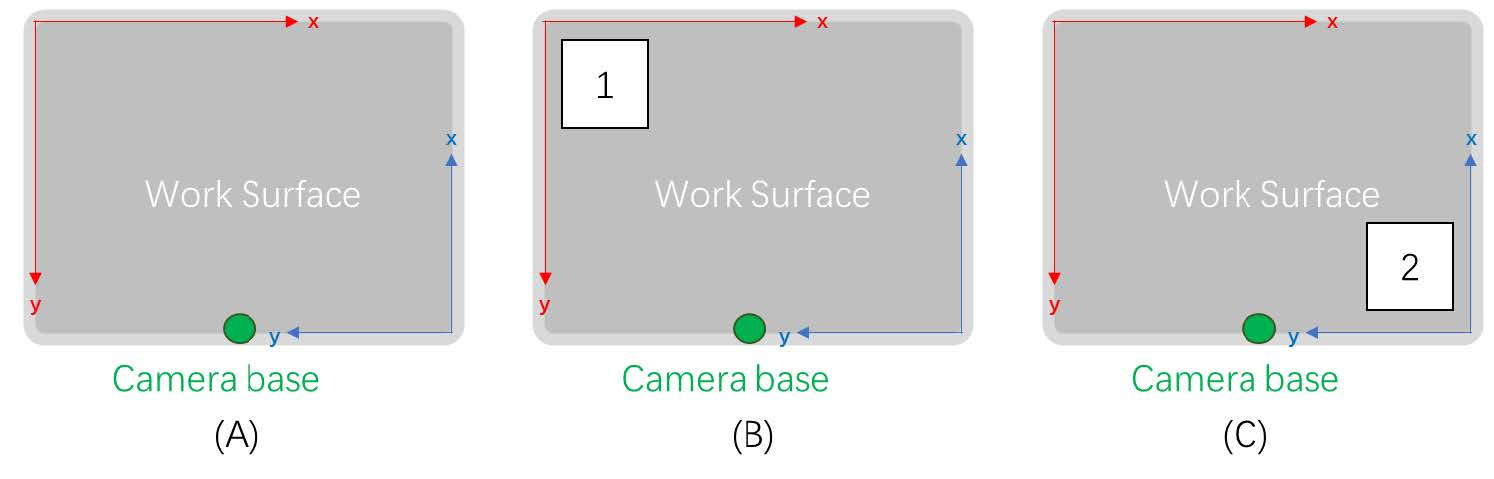
\includegraphics[scale=0.8]{image/lab7_register.jpg}
	\caption{\figlbl{lab6register} Registering two positions to find image-robot relationship}
\end{figure}

\begin{itemize}
    \item Transform Image (Pixel) Coordinates to Robotic Reference Frame
    \begin{itemize}
        \item Define relationship between the robot base frame and the pixel coordinate frame as
        illustrated by the red and blue axes, respectively.
        \item Move robot to Region 1: pixel coordinates $(x_1,y_1)$; register the robot coordinates as $(x_1',y_1')$.
        \item Move robot to Region 2: pixel coordinates $(x_2,y_2)$; register the robot coordinates as $(x_2',y_2')$
        \item Obtain the ratio that map $(x,y)$ to $(x',y')$ as define below:
        \begin{equation}
            \begin{aligned}
            &x_{ratio}=\left(x_{2}^{\prime}-x_{1}^{\prime}\right) /\left(y_{2}-y_{1}\right) \\
            &y_{ratio}=\left(y_{2}^{\prime}-y_{1}^{\prime}\right) /\left(x_{2}-x_{1}\right)
            \end{aligned}
        \end{equation}
        \begin{equation}
            \begin{aligned}
            &x^{\prime}=x^{\prime}_1+x_{ratio} *\left(y-y_{1}\right) \\
            &y^{\prime}=y^{\prime}_1+y_{ratio} *\left(x-x_{1}\right)
            \end{aligned}
        \end{equation}
    \end{itemize}
    \item Classify Objects and Compute Pose (Lab 5: Image Processing)
    \begin{itemize}
        \item Label the objects and
        \item Compute their center positions and orientation in the scene
    \end{itemize}
    \begin{figure}
        \centering
            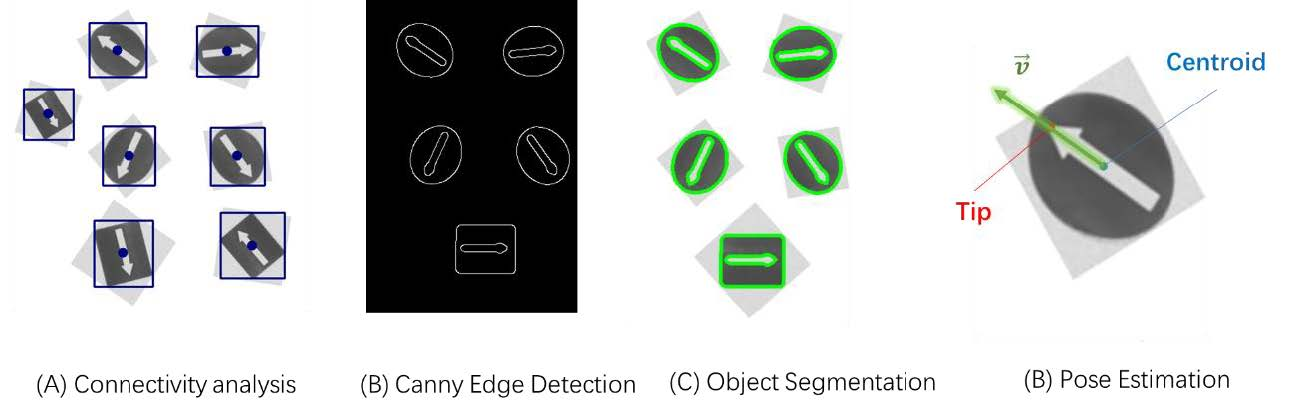
\includegraphics[scale=1]{image/lab7_pose.jpg}
        \caption{\figlbl{lab6process} Image processing to classify and localize object in camera scene}
    \end{figure}

    \item Move Robot using on Transformed Coordinates
    Move robot arm from one position to another as you have done in Lab 4 (inverse kinematics)
    with the Transformed Coordinates,
    \begin{itemize}
        \item Locate objects and check their label as in the image
        \item Transform coordinates to robot coordinate system
        \item Move to pick (suction grip) object from the unsorted tray as should in \figref{lab6flow}
        \item Move to sort objects into specific pose in the sorted tray as shown in \figref{lab6flow}
    \end{itemize}
\end{itemize}

\begin{figure}
	\centering
		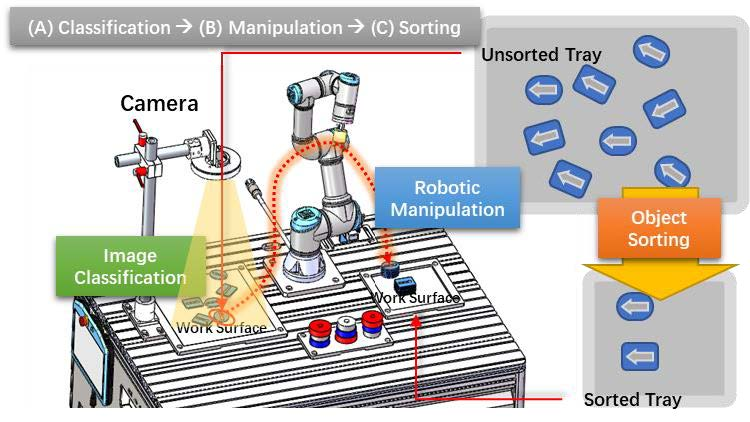
\includegraphics[scale=1]{image/lab6_table.jpg}
	\caption{\figlbl{lab6flow} Image processing to classify and localize object in camera scene}
\end{figure}


\section{Debugging}
This lab can be a bit tricky to work through as several parts require trial and error.  Here are some suggestions:
\begin{itemize}
    \item Approach the lab sequentially and make sure you get good results at each step.
    \item Comment out parts that you are not currently using (Don't forget the uncomment them though...)
\end{itemize}


\section{Report}
This lab does not require a formal lab report - only the submission of your code.  You should a submit a document to \href{https://learn.intl.zju.edu.cn/}{Blackboard} containing all of the files that you edited to complete the lab.  This will be submitted to \href{https://learn.intl.zju.edu.cn/}{Blackboard} as in the past.

\section{Demo}
Your TA will require you to run your program twice, each time with different initial block positions and verify that your program can locate the blocks and place them in the correct location.  You will also demonstrate that suction feedback is working.

\section{Grading}
\begin{itemize}
\item 100 points, successful demonstration and submission of the code. (No code = 0 points)
\end{itemize}


% \section{Tentative Due Dates - Fall 2020}
% Lab 5 demonstration will be due by 5PM on Wednesday, December 16.  Code must be submitted on \href{www.gradescope.com}{GradeScope}, by midnight that same day.  Note that each TA will only have a limited number of office hours prior to this time, so you should plan ahead to meet this deadline.
